\documentclass[border=6pt]{standalone}
\usepackage{amsmath}
\usepackage{amssymb}
\usepackage{tikz}
\usepackage{pgfplots}
\pgfplotsset{compat=1.18}
\usetikzlibrary{arrows.meta,calc,positioning}
\begin{document}
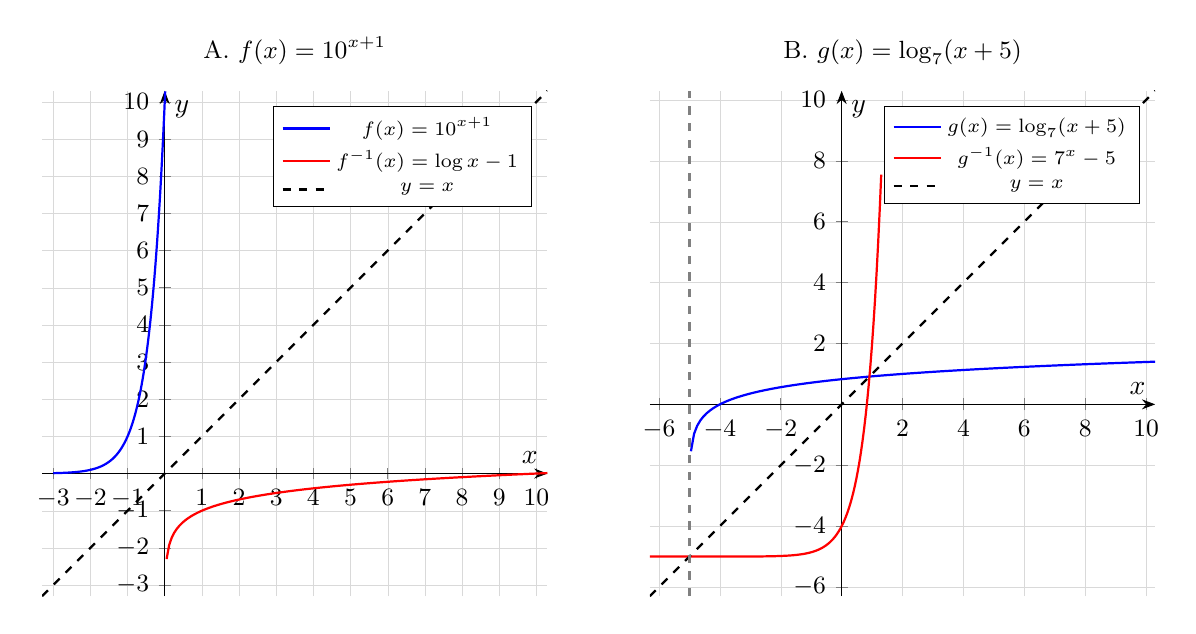
\begin{tikzpicture}
\begin{axis}[name=ax1,
    axis lines = middle,
    xlabel = {$x$}, ylabel = {$y$},
    grid=both,
    grid style={line width=.1pt, draw=gray!30},
    axis line style={-Stealth},
    legend style={font=\scriptsize},
    tick label style={font=\small},
    xmin=-3.3, xmax=10.3, ymin=-3.3, ymax=10.3,
    xtick={-3,-2,-1,0,1,2,3,4,5,6,7,8,9,10},
    ytick={-3,-2,-1,0,1,2,3,4,5,6,7,8,9,10},
    width=8cm, height=8cm,
    title={\small A. $f(x)=10^{x+1}$},
    legend pos=north east,
]
\addplot[domain=-3:0.3, samples=150, restrict y to domain=-3.3:10.3, thick, blue] {10^(x+1)};
\addlegendentry{$f(x)=10^{x+1}$}
\addplot[domain=0.05:10.3, samples=150, restrict y to domain=-3.3:10.3, thick, red] {ln(x)/ln(10)-1};
\addlegendentry{$f^{-1}(x)=\log x -1$}
\addplot[domain=-3.3:10.3, samples=2, thick, black, dashed] {x};
\addlegendentry{$y=x$}
\end{axis}
\begin{axis}[at={(ax1.south east)}, anchor=south west, xshift=1.3cm,
    axis lines = middle,
    xlabel = {$x$}, ylabel = {$y$},
    grid=both,
    grid style={line width=.1pt, draw=gray!30},
    axis line style={-Stealth},
    legend style={font=\scriptsize},
    tick label style={font=\small},
    xmin=-6.3, xmax=10.3, ymin=-6.3, ymax=10.3,
    xtick={-6,-4,-2,0,2,4,6,8,10},
    ytick={-6,-4,-2,0,2,4,6,8,10},
    width=8cm, height=8cm,
    title={\small B. $g(x)=\log_7(x+5)$},
    legend pos=north east,
]
\addplot[domain=-4.95:10.3, samples=150, restrict y to domain=-6.3:10.3, thick, blue] {ln(x+5)/ln(7)};
\addlegendentry{$g(x)=\log_7(x+5)$}
\addplot[domain=-6.3:1.3, samples=150, restrict y to domain=-6.3:10.3, thick, red] {7^x-5};
\addlegendentry{$g^{-1}(x)=7^x-5$}
\addplot[domain=-6.3:10.3, samples=2, thick, black, dashed] {x};
\addlegendentry{$y=x$}
\draw[dashed, gray, thick] (axis cs:-5,-6.3) -- (axis cs:-5,10.3);
\node[anchor=north, font=\scriptsize, gray] at (axis cs:-5,-6.1) {$x=-5$};
\end{axis}
\end{tikzpicture}
\end{document}
